
%% bare_conf.tex
%% V1.3
%% 2007/01/11
%% by Michael Shell
%% See:
%% http://www.michaelshell.org/
%% for current contact information.
%%
%% This is a skeleton file demonstrating the use of IEEEtran.cls
%% (requires IEEEtran.cls version 1.7 or later) with an IEEE conference paper.
%%
%% Support sites:
%% http://www.michaelshell.org/tex/ieeetran/
%% http://www.ctan.org/tex-archive/macros/latex/contrib/IEEEtran/
%% and
%% http://www.ieee.org/

%%*************************************************************************
%% Legal Notice:
%% This code is offered as-is without any warranty either expressed or
%% implied; without even the implied warranty of MERCHANTABILITY or
%% FITNESS FOR A PARTICULAR PURPOSE!
%% User assumes all risk.
%% In no event shall IEEE or any contributor to this code be liable for
%% any damages or losses, including, but not limited to, incidental,
%% consequential, or any other damages, resulting from the use or misuse
%% of any information contained here.
%%
%% All comments are the opinions of their respective authors and are not
%% necessarily endorsed by the IEEE.
%%
%% This work is distributed under the LaTeX Project Public License (LPPL)
%% ( http://www.latex-project.org/ ) version 1.3, and may be freely used,
%% distributed and modified. A copy of the LPPL, version 1.3, is included
%% in the base LaTeX documentation of all distributions of LaTeX released
%% 2003/12/01 or later.
%% Retain all contribution notices and credits.
%% ** Modified files should be clearly indicated as such, including  **
%% ** renaming them and changing author support contact information. **
%%
%% File list of work: IEEEtran.cls, IEEEtran_HOWTO.pdf, bare_adv.tex,
%%                    bare_conf.tex, bare_jrnl.tex, bare_jrnl_compsoc.tex
%%*************************************************************************

% *** Authors should verify (and, if needed, correct) their LaTeX system  ***
% *** with the testflow diagnostic prior to trusting their LaTeX platform ***
% *** with production work. IEEE's font choices can trigger bugs that do  ***
% *** not appear when using other class files.                            ***
% The testflow support page is at:
% http://www.michaelshell.org/tex/testflow/



% Note that the a4paper option is mainly intended so that authors in
% countries using A4 can easily print to A4 and see how their papers will
% look in print - the typesetting of the document will not typically be
% affected with changes in paper size (but the bottom and side margins will).
% Use the testflow package mentioned above to verify correct handling of
% both paper sizes by the user's LaTeX system.
%
% Also note that the "draftcls" or "draftclsnofoot", not "draft", option
% should be used if it is desired that the figures are to be displayed in
% draft mode.
%
%\documentclass[conference]{IEEEtran}
\documentclass[10pt, conference, compsocconf]{IEEEtran}
% Add the compsoc option for Computer Society conferences.
%
% If IEEEtran.cls has not been installed into the LaTeX system files,
% manually specify the path to it like:
% \documentclass[conference]{../sty/IEEEtran}


% Some very useful LaTeX packages include:
% (uncomment the ones you want to load)


% *** MISC UTILITY PACKAGES ***
%
\usepackage{ifpdf}
% Heiko Oberdiek's ifpdf.sty is very useful if you need conditional
% compilation based on whether the output is pdf or dvi.
% usage:
% \ifpdf
%   % pdf code
% \else
%   % dvi code
% \fi
% The latest version of ifpdf.sty can be obtained from:
% http://www.ctan.org/tex-archive/macros/latex/contrib/oberdiek/
% Also, note that IEEEtran.cls V1.7 and later provides a builtin
% \ifCLASSINFOpdf conditional that works the same way.
% When switching from latex to pdflatex and vice-versa, the compiler may
% have to be run twice to clear warning/error messages.


\ifCLASSOPTIONcompsoc
  % IEEE Computer Society needs nocompress option
  % requires cite.sty v4.0 or later (November 2003)
  \usepackage[nocompress]{cite}
\else
  % normal IEEE
  \usepackage{cite}
\fi




% *** CITATION PACKAGES ***
\usepackage{url}
\usepackage{cite}
\usepackage[numbers,square, comma, sort&compress]{natbib}
%\usepackage[comma]{natbib}
% cite.sty was written by Donald Arseneau
% V1.6 and later of IEEEtran pre-defines the format of the cite.sty package
% \cite{} output to follow that of IEEE. Loading the cite package will
% result in citation numbers being automatically sorted and properly
% "compressed/ranged". e.g., [1], [9], [2], [7], [5], [6] without using
% cite.sty will become [1], [2], [5]--[7], [9] using cite.sty. cite.sty's
% \cite will automatically add leading space, if needed. Use cite.sty's
% noadjust option (cite.sty V3.8 and later) if you want to turn this off.
% cite.sty is already installed on most LaTeX systems. Be sure and use
% version 4.0 (2003-05-27) and later if using hyperref.sty. cite.sty does
% not currently provide for hyperlinked citations.
% The latest version can be obtained at:
% \cite{http://www.ctan.org/tex-archive/macros/latex/contrib/cite/}
% The documentation is contained in the cite.sty file itself.


\usepackage[T1]{fontenc}


% *** GRAPHICS RELATED PACKAGES ***
%
\ifCLASSINFOpdf
  \usepackage[pdftex]{graphicx}
  % declare the path(s) where your graphic files are
  % \graphicspath{{../pdf/}{../jpeg/}}
  % and their extensions so you won't have to specify these with
  % every instance of \includegraphics
  % \DeclareGraphicsExtensions{.pdf,.jpeg,.png}
\else
  % or other class option (dvipsone, dvipdf, if not using dvips). graphicx
  % will default to the driver specified in the system graphics.cfg if no
  % driver is specified.
  % \usepackage[dvips]{graphicx}
  % declare the path(s) where your graphic files are
  % \graphicspath{{../eps/}}
  % and their extensions so you won't have to specify these with
  % every instance of \includegraphics
  % \DeclareGraphicsExtensions{.eps}
\fi
% graphicx was written by David Carlisle and Sebastian Rahtz. It is
% required if you want graphics, photos, etc. graphicx.sty is already
% installed on most LaTeX systems. The latest version and documentation can
% be obtained at:
% http://www.ctan.org/tex-archive/macros/latex/required/graphics/
% Another good source of documentation is "Using Imported Graphics in
% LaTeX2e" by Keith Reckdahl which can be found as epslatex.ps or
% epslatex.pdf at: http://www.ctan.org/tex-archive/info/
%
% latex, and pdflatex in dvi mode, support graphics in encapsulated
% postscript (.eps) format. pdflatex in pdf mode supports graphics
% in .pdf, .jpeg, .png and .mps (metapost) formats. Users should ensure
% that all non-photo figures use a vector format (.eps, .pdf, .mps) and
% not a bitmapped formats (.jpeg, .png). IEEE frowns on bitmapped formats
% which can result in "jaggedy"/blurry rendering of lines and letters as
% well as large increases in file sizes.
%
% You can find documentation about the pdfTeX application at:
% http://www.tug.org/applications/pdftex





% *** MATH PACKAGES ***
%
\usepackage[cmex10]{amsmath}
% A popular package from the American Mathematical Society that provides
% many useful and powerful commands for dealing with mathematics. If using
% it, be sure to load this package with the cmex10 option to ensure that
% only type 1 fonts will utilized at all point sizes. Without this option,
% it is possible that some math symbols, particularly those within
% footnotes, will be rendered in bitmap form which will result in a
% document that can not be IEEE Xplore compliant!
%
% Also, note that the amsmath package sets \interdisplaylinepenalty to 10000
% thus preventing page breaks from occurring within multiline equations. Use:
%\interdisplaylinepenalty=2500
% after loading amsmath to restore such page breaks as IEEEtran.cls normally
% does. amsmath.sty is already installed on most LaTeX systems. The latest
% version and documentation can be obtained at:
% http://www.ctan.org/tex-archive/macros/latex/required/amslatex/math/





% *** SPECIALIZED LIST PACKAGES ***
%
%\usepackage{algorithm2e}
% algorithmic.sty was written by Peter Williams and Rogerio Brito.
% This package provides an algorithmic environment fo describing algorithms.
% You can use the algorithmic environment in-text or within a figure
% environment to provide for a floating algorithm. Do NOT use the algorithm
% floating environment provided by algorithm.sty (by the same authors) or
% algorithm2e.sty (by Christophe Fiorio) as IEEE does not use dedicated
% algorithm float types and packages that provide these will not provide
% correct IEEE style captions. The latest version and documentation of
% algorithmic.sty can be obtained at:
% http://www.ctan.org/tex-archive/macros/latex/contrib/algorithms/
% There is also a support site at:
% http://algorithms.berlios.de/index.html
% Also of interest may be the (relatively newer and more customizable)
% algorithmicx.sty package by Szasz Janos:
% http://www.ctan.org/tex-archive/macros/latex/contrib/algorithmicx/
\usepackage{algorithm} %format of the algorithm
\usepackage{algorithmic} %format of the algorithm
\usepackage{multirow} %multirow for format of table
\usepackage{amsmath}
\usepackage{xcolor}
%\usepackage{algpseudocode}
\renewcommand{\algorithmicrequire}{\textbf{Input:}}
\renewcommand{\algorithmicensure}{\textbf{Output:}}
\setlength{\textfloatsep}{5pt plus 1.0pt minus 2.0pt}

% *** ALIGNMENT PACKAGES ***
%
\usepackage{array}
% Frank Mittelbach's and David Carlisle's array.sty patches and improves
% the standard LaTeX2e array and tabular environments to provide better
% appearance and additional user controls. As the default LaTeX2e table
% generation code is lacking to the point of almost being broken with
% respect to the quality of the end results, all users are strongly
% advised to use an enhanced (at the very least that provided by array.sty)
% set of table tools. array.sty is already installed on most systems. The
% latest version and documentation can be obtained at:
% http://www.ctan.org/tex-archive/macros/latex/required/tools/


\usepackage{mdwmath}
\usepackage{mdwtab}
% Also highly recommended is Mark Wooding's extremely powerful MDW tools,
% especially mdwmath.sty and mdwtab.sty which are used to format equations
% and tables, respectively. The MDWtools set is already installed on most
% LaTeX systems. The lastest version and documentation is available at:
% http://www.ctan.org/tex-archive/macros/latex/contrib/mdwtools/


% IEEEtran contains the IEEEeqnarray family of commands that can be used to
% generate multiline equations as well as matrices, tables, etc., of high
% quality.


%\usepackage{eqparbox}
% Also of notable interest is Scott Pakin's eqparbox package for creating
% (automatically sized) equal width boxes - aka "natural width parboxes".
% Available at:
% http://www.ctan.org/tex-archive/macros/latex/contrib/eqparbox/





% *** SUBFIGURE PACKAGES ***
\usepackage[tight,footnotesize]{subfigure}
% subfigure.sty was written by Steven Douglas Cochran. This package makes it
% easy to put subfigures in your figures. e.g., "Figure 1a and 1b". For IEEE
% work, it is a good idea to load it with the tight package option to reduce
% the amount of white space around the subfigures. subfigure.sty is already
% installed on most LaTeX systems. The latest version and documentation can
% be obtained at:
% http://www.ctan.org/tex-archive/obsolete/macros/latex/contrib/subfigure/
% subfigure.sty has been superceeded by subfig.sty.
\usepackage{graphicx}
\usepackage{subfloat}
\usepackage{float}

\usepackage{caption}
%\captionsetup[table]{belowskip=18pt, aboveskip = 5pt}
%\usepackage[font=footnotesize]{subfig}
% subfig.sty, also written by Steven Douglas Cochran, is the modern
% replacement for subfigure.sty. However, subfig.sty requires and
% automatically loads Axel Sommerfeldt's caption.sty which will override
% IEEEtran.cls handling of captions and this will result in nonIEEE style
% figure/table captions. To prevent this problem, be sure and preload
% caption.sty with its "caption=false" package option. This is will preserve
% IEEEtran.cls handing of captions. Version 1.3 (2005/06/28) and later
% (recommended due to many improvements over 1.2) of subfig.sty supports
% the caption=false option directly:
%\usepackage[caption=false,font=footnotesize]{subfig}
%
% The latest version and documentation can be obtained at:
% http://www.ctan.org/tex-archive/macros/latex/contrib/subfig/
% The latest version and documentation of caption.sty can be obtained at:
% http://www.ctan.org/tex-archive/macros/latex/contrib/caption/




% *** FLOAT PACKAGES ***
%
%\usepackage{fixltx2e}
% fixltx2e, the successor to the earlier fix2col.sty, was written by
% Frank Mittelbach and David Carlisle. This package corrects a few problems
% in the LaTeX2e kernel, the most notable of which is that in current
% LaTeX2e releases, the ordering of single and double column floats is not
% guaranteed to be preserved. Thus, an unpatched LaTeX2e can allow a
% single column figure to be placed prior to an earlier double column
% figure. The latest version and documentation can be found at:
% http://www.ctan.org/tex-archive/macros/latex/base/



%\usepackage{stfloats}
% stfloats.sty was written by Sigitas Tolusis. This package gives LaTeX2e
% the ability to do double column floats at the bottom of the page as well
% as the top. (e.g., "\begin{figure*}[!b]" is not normally possible in
% LaTeX2e). It also provides a command:
%\fnbelowfloat
% to enable the placement of footnotes below bottom floats (the standard
% LaTeX2e kernel puts them above bottom floats). This is an invasive package
% which rewrites many portions of the LaTeX2e float routines. It may not work
% with other packages that modify the LaTeX2e float routines. The latest
% version and documentation can be obtained at:
% http://www.ctan.org/tex-archive/macros/latex/contrib/sttools/
% Documentation is contained in the stfloats.sty comments as well as in the
% presfull.pdf file. Do not use the stfloats baselinefloat ability as IEEE
% does not allow \baselineskip to stretch. Authors submitting work to the
% IEEE should note that IEEE rarely uses double column equations and
% that authors should try to avoid such use. Do not be tempted to use the
% cuted.sty or midfloat.sty packages (also by Sigitas Tolusis) as IEEE does
% not format its papers in such ways.





% *** PDF, URL AND HYPERLINK PACKAGES ***
%
\usepackage{url}
% url.sty was written by Donald Arseneau. It provides better support for
% handling and breaking URLs. url.sty is already installed on most LaTeX
% systems. The latest version can be obtained at:
% http://www.ctan.org/tex-archive/macros/latex/contrib/misc/
% Read the url.sty source comments for usage information. Basically,
% \url{my_url_here}.





% *** Do not adjust lengths that control margins, column widths, etc. ***
% *** Do not use packages that alter fonts (such as pslatex).         ***
% There should be no need to do such things with IEEEtran.cls V1.6 and later.
% (Unless specifically asked to do so by the journal or conference you plan
% to submit to, of course. )


% correct bad hyphenation here
\hyphenation{op-tical net-works semi-conduc-tor}


\begin{document}
\nocite{*}
%
% paper title
% can use linebreaks \\ within to get better formatting as desired
\title{Assignment1: Supervised Learning Report}


% author names and affiliations
% use a multiple column layout for up to three different
% affiliations
\author{\IEEEauthorblockN{Liang Xu}
	\IEEEauthorblockA{College of Computing\\
		Georgia Institute of Technology\\
}}

% conference papers do not typically use \thanks and this command
% is locked out in conference mode. If really needed, such as for
% the acknowledgment of grants, issue a \IEEEoverridecommandlockouts
% after \documentclass

% for over three affiliations, or if they all won't fit within the width
% of the page, use this alternative format:
%
%\author{\IEEEauthorblockN{Michael Shell\IEEEauthorrefmark{1},
%Homer Simpson\IEEEauthorrefmark{2},
%James Kirk\IEEEauthorrefmark{3},
%Montgomery Scott\IEEEauthorrefmark{3} and
%Eldon Tyrell\IEEEauthorrefmark{4}}
%\IEEEauthorblockA{\IEEEauthorrefmark{1}School of Electrical and Computer Engineering\\
%Georgia Institute of Technology,
%Atlanta, Georgia 30332--0250\\ Email: see http://www.michaelshell.org/contact.html}
%\IEEEauthorblockA{\IEEEauthorrefmark{2}Twentieth Century Fox, Springfield, USA\\
%Email: homer@thesimpsons.com}
%\IEEEauthorblockA{\IEEEauthorrefmark{3}Starfleet Academy, San Francisco, California 96678-2391\\
%Telephone: (800) 555--1212, Fax: (888) 555--1212}
%\IEEEauthorblockA{\IEEEauthorrefmark{4}Tyrell Inc., 123 Replicant Street, Los Angeles, California 90210--4321}}




% use for special paper notices
%\IEEEspecialpapernotice{(Invited Paper)}




% make the title area
\maketitle


\begin{abstract}
	%\boldmath
This is the assignment 1: Supervised Learning Algorithm report for CS-7641 Machine Learning class in Georgia Tech. The purpose of this report is to develop some understanding of techniques in supervised learning. In this report, five different supervised learning algorithms have been applied to two different datasets. The algorithm includes decision tree with some of pruning, neural networks, boosting, support vector machines, and k-nearest neighbors.There will be various circumstances condition to test the algorithm performance. The programming language used is Python3 and all the algorithms are implemented by using scikit-learn machine learning library. 
\end{abstract}
% IEEEtran.cls defaults to using nonbold math in the Abstract.
% This preserves the distinction between vectors and scalars. However,
% if the conference you are submitting to favors bold math in the abstract,
% then you can use LaTeX's standard command \boldmath at the very start
% of the abstract to achieve this. Many IEEE journals/conferences frown on
% math in the abstract anyway.


%% no keywords
%\vspace{1em}
%
%\noindent \textbf{Keywords:}\quad Flash memory, Out-of-place update, Read cache, LRU.
% \vspace{1em}




% For peer review papers, you can put extra information on the cover
% page as needed:
% \ifCLASSOPTIONpeerreview
% \begin{center} \bfseries EDICS Category: 3-BBND \end{center}
% \fi
%
% For peerreview papers, this IEEEtran command inserts a page break and
% creates the second title. It will be ignored for other modes.
\IEEEpeerreviewmaketitle

\section{Introduction}
Supervised learning is the machine learning task of inferring a function from labeled training data\cite{mohri2012foundations}. The training data consist of pair input objectives and output classes. The supervised learning algorithm, for example, decision tree and SVM, analyzes the training data and "Learn" a meta-model to represent the relationship between input parameters and output classes. This model will be used to map for mapping new or even brand new instances.  

In this report, there will be two data sets used to make a comparison between five different supervised learning algorithms. The comparison between the algorithms will be in detail. Training and testing error rates will be obtained, learning graph and model complexity will be plotted. A detailed result analysis will be the main component of this report. 

This report is organized as follows: section 2 describe the two data sets. Section 3 presents different algorithm's results. Section 4 discusses the characteristic of each result and detailed comparison 

\section{Data sets}
Both of the data set are come from UCI Machine Learning Repository. One is mushroom data set\cite{Mushroom}, and another is bank marking data set\cite{bank}. Table \ref{tab:1} is a basic summary of those two data sets. Both of the data sets can be used as binary classification. For mushroom data, we classify is poisonous oe edible, for bank data we predict the client will be subscribe a term deposit. Both of the data sets are from real world, not generated data for particular machine learning study. Mush room data is small and old, bank data is recent data.

\begin{table}[h]
	\centering
	\caption{Data Sets Summary}
	\label{tab:1}
	\begin{tabular}{|l|c|c|c|l|l|}
		\hline
		Data Set & \multicolumn{1}{l|}{Instances} & \multicolumn{1}{l|}{Attributes} & \multicolumn{1}{l|}{Result Class} & Date & Tasks          \\ \hline
		Mushroom & 8124                           & 22                              & 2(E/P)                            & 1987 & Classify \\ \hline
		Bank     & 45211                          & 17                              & 2(Y/N)                            & 2012 & Classify \\ \hline
	\end{tabular}
\end{table}

\subsection[]{Mushroom Data Set}
Mushroom records are drawn from The Audubon Society Field Guide to North
American Mushrooms (1981). This dataset includes descriptions of hypothetical samples
corresponding to 23 species of gilled mushrooms in the Agaricus. Each species is identified as definitely edible, definitely poisonous.
The dataset consists of 2 classes, edible and poisonous. The number of edible 4208(51.8\%), and the number of poisonous have 3916(48.2\%) total has 8124 instances. So we can assume the two datasets have an equal number of samples, so random guess will achieve 50\% accuracy.\\
 The reason for me to choose this dataset because one of the articles to use this data to teach decision tree\cite{decisionTree}. I found this data is quite good for beginners. The result is evenly distributed and data size is not too big or too small, also the result quite good. 
\begin{table}[h]
	\centering
	\caption{Mushroom Dataset Summary}
	\label{tab:2}
\begin{tabular}{|c|c|c|c|c|c|c|}
	\hline
	         & class & cap-shape & bruises & veil-type & odor & cap-surf    \\ \hline
	count    & 8124  & 8124      & 8124    & 8124      & 8124 & 8124        \\ \hline
	unique   & 2     & 6         & 2       & 1         & 9    & 4           \\ \hline
	top      & e     & x         & f       & p         & n    & y           \\ \hline
	freq     & 4208  & 3656      & 4748    & 8124      & 3528 & 3244        \\ \hline
\end{tabular}
\end{table}

Table \ref{tab:2} is a summary about mushroom data set. 6 features from 23 features have been selected to show the summary. Some of the features are quite interesting for classification. For example, 'bruises' feature has 2 classes, and the top frequency is 4748, which is quite similar to 'Class' feature. However, from Figure \ref{fig:1} (right side) the distribution of 'bruises' v.s 'Class', we found out this feature does not have a high confidence with what we expect, we can say 't' class have a high probability can be classified as 'e' . For feature 'veil-type', it only has one class 'p', this feature will not give us any information to determine the mushroom is an 'e' or 'p'. Let check the 'odor' feature, this feature have 9 classes, from figure \ref{fig:1} (left), we can easily determine class 'e' is on the left side and 'p' on the right side.So, even though the feature have the same number of classes with the final classification result, it does not mean it a good feature to determine the class.\\
Figure \ref{fig:mushroomSummary} is the summary of the mushroom data set. From this summary graph we can easily found some of the features are quite easy to determine the class of a particular mush room. Figure \ref{fig:mushroomimportance} is a feature importance for each feature. In order to make our machine learning problem become harder I removed some of the killing features {'habitat','population','gill-color','spore-print-color','odor','gill-size','stalk-root','gill-spacing','cap-color'}. So in the following report, only 12 features have been used. 
% Figure
\begin{figure}[h]
	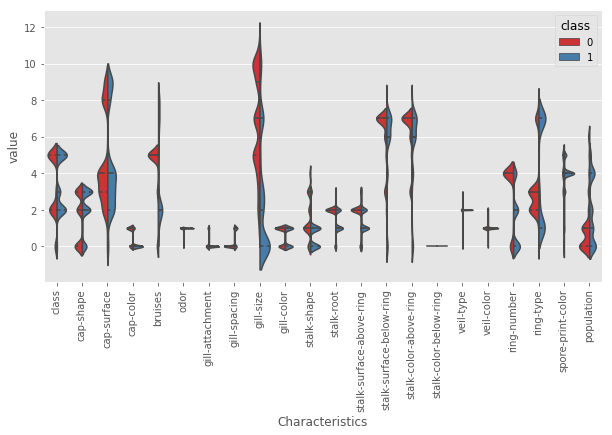
\includegraphics[scale = 0.4]{image/mushroomSummary.png}
	\caption{Mushroom Data Feature Distribution Summary}
	\label{fig:mushroomSummary}
\end{figure}

\begin{figure}[h]
	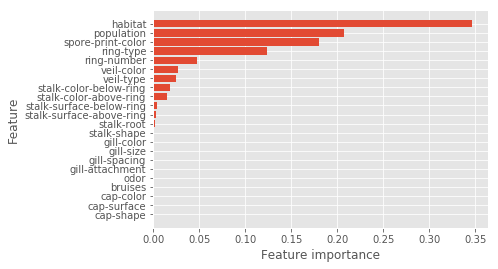
\includegraphics[scale = 0.4]{image/mushroomFullFeature_important.png}
	\caption{Mushroom Data Feature Importance for Decision Tree}
	\label{fig:mushroomimportance}
\end{figure}

\begin{figure}[h]
	\hfill
	\centering
	\subfigure{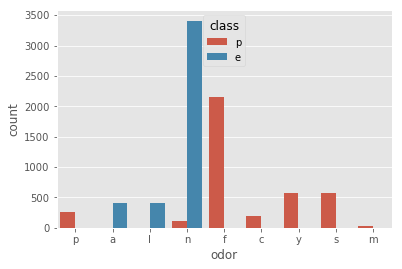
\includegraphics[width=4cm]{image/odor.png}}
	\hfill
	\subfigure{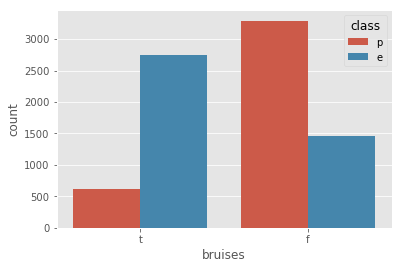
\includegraphics[width=4cm]{image/bruises.png}}
	\hfill
	\caption{Odor and Bruises distributions}
	\label{fig:1}
	
\end{figure}

\begin{figure}[h]
	\hfill
	\centering
	\subfigure{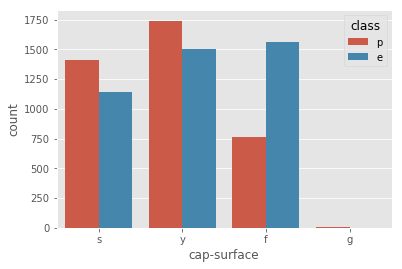
\includegraphics[width=4cm]{image/cap-surface.png}}
	\hfill
	\subfigure{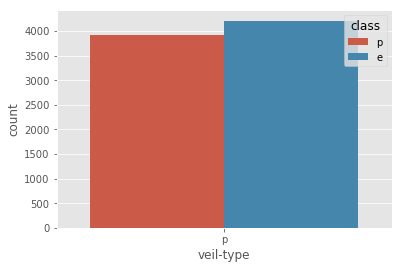
\includegraphics[width=4cm]{image/veil-type.png}}
	\hfill
	\caption{Cap-surface and Veil-type distributions}
	\label{fig:2}
	
\end{figure}
 

\subsection[]{Bank Marketing Data Set}
The data is related with direct marketing campaigns of a Portuguese banking institution. The marketing campaigns were based on phone calls. Often, more than one contact to the same client was required, in order to access if the product (bank term deposit) would be ('yes') or not ('no') subscribed \cite{bank}.
The bank dataset contains both type variables "Categorical" and "Numerical". for example, age and balance are both 'Numerical', and job and marital both "Categorical".\\
Figure \ref{fig:bankSummary} is the summary for different features distribution. From this summary, we can see the data distribution is hard to make a direct guess the result, which means the problem is a little bit hard for human. 
\begin{figure}[h]
	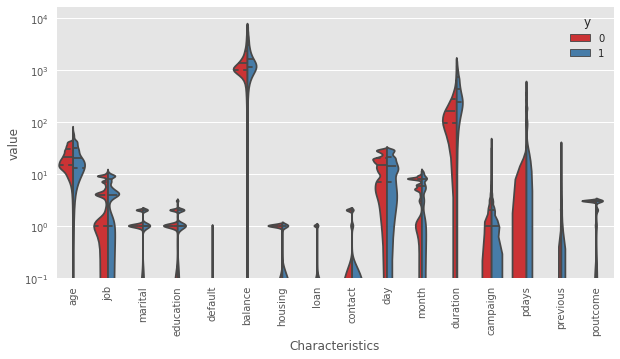
\includegraphics[scale = 0.4]{image/bankSummary.png}
	\caption{Bank Data Feature Distribution Summary}
	\label{fig:bankSummary}
\end{figure}
\begin{figure}[h]
	\hfill
	\centering
	\subfigure{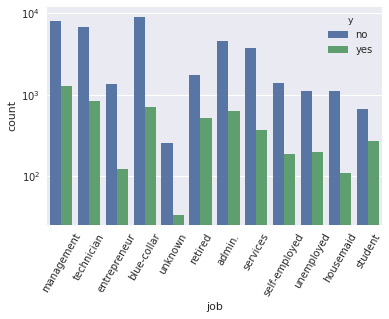
\includegraphics[width=4cm]{image/job.png}}
	\hfill
	\subfigure{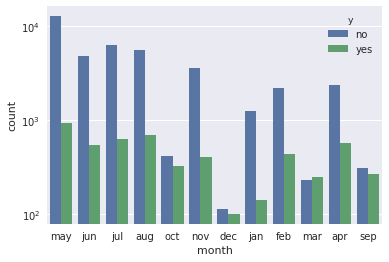
\includegraphics[width=4cm]{image/mounth.png}}
	\hfill
	\caption{Categorical distribution example}
	\label{fig:3}
	
\end{figure}

\begin{figure}[h]
	\hfill
	\centering
	\subfigure{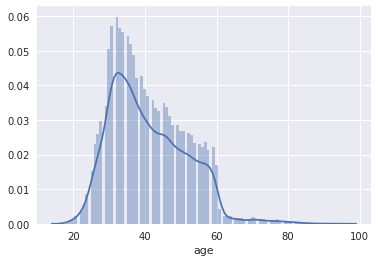
\includegraphics[width=4cm]{image/age.png}}
	\hfill
	\subfigure{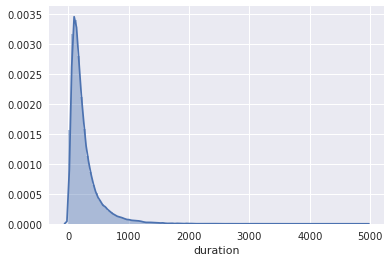
\includegraphics[width=4cm]{image/duration.png}}
	\hfill
	\caption{Numerical data example}
	\label{fig:4}
	
\end{figure}

Above figure are the display of different category and numerical data. For job and mouthes distribution, the y-axis uses a log scale. Because, in this data set, the number of 'yes' class only have 5289(11.7\%), and  'no' have 39922(88.3\%), so the dataset is highly unbalanced.
The reason I chose this data is that of its combination with the Numerical and Categorical feature, which make the algorithm a little bit different compared with the first one. Also, the data set is unbalanced in terms of the success rate. Only 11.7\% of the data classified as "yes". I want to see how machine learning algorithm handles this.

\section{Supervised learning Algorithm Result}
In this section, five different machine learning technique will be implemented to the two datasets mentioned in the above paragraph. All the algorithms are directly from the scikit-learn: machine learning library in Python. There is python note book contains all the plots and code. 
To evaluate the five classification problem, the dataset has been separated to 80/20 for training and testing. For comparison, five different algorithm will be using the same tranning dataset and same testing set. 
\subsection{Decision Tree}
Decision Trees (DTs) are a non-parametric supervised learning method used for classification and regression. The goal is to create a model that predicts the value of a target variable by learning simple decision rules inferred from the data features.\\
In this part of the report, I will show some of the accuracy result and some analysis between the two data set. 
\subsubsection{Decision Tree for Mushroom Dataset}
The result for mushroom data is very good, even though not all the features have been used for classification. The best testing score we can get is 96.18\%, by using 13 layer depth and 13 features decision tree. \\
Fist let us find out how important each feature used in the decision tree. Figure \ref{fig:mushroomimportance} is the feature importance distribution for the best-scored decision tree. Figure \ref{fig:tree} is the tree for this model, for simplicity, I just cut off this tree to 2 level. From the importance and tree figure, we can easily find out the 'ring-type' is on the top of the tree, because it has the largest 'gini' index. 

\begin{figure}[h]
	\centering
	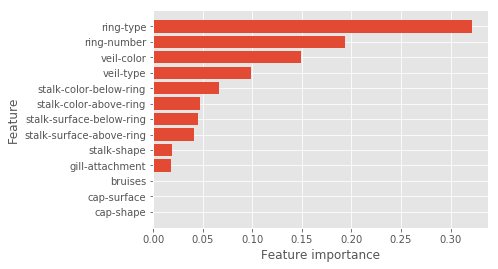
\includegraphics[scale = 0.4]{image/decMushRoomImportant.png}
	\caption{Feature Importance for Mushroom Dataset }
	\label{fig:mushFeature}
\end{figure}

\begin{figure}[h]
	\centering
	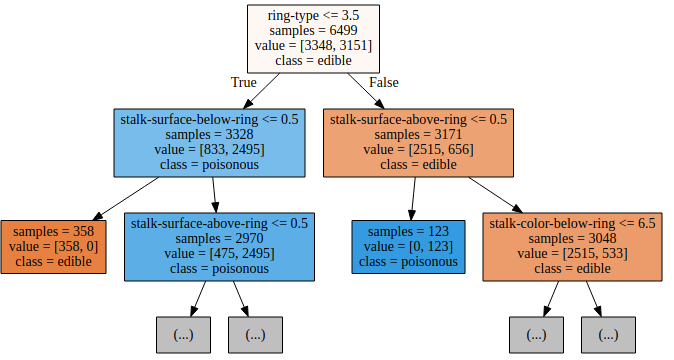
\includegraphics[scale = 0.35]{image/decisionTree.png}
	\caption{Best Decision Tree for Mushroom Dataset }
	\label{fig:tree}
\end{figure}
Let us check the learning rate of this algorithm. Figure \ref{fig:treelearn} is the testing set accuracy compare with the number of samples. For this figure, we can easily assume the accuracy of the model is increasing dramatically from 1 to 100, then from 100 to 300 the accuracy increase rate become slow. Finally, the accuracy increasing rate become very slow. This means the heavy learning in the begin of the process, as the amount data increased, the learning become slow. \\
Form this figure, we can also found out, with the training data increased the testing accuracy is not decrease, which means the model is over fitting with too mush data. I will use cross validation method to test what I have proposed here. \\ 
In the Figure \ref{fig:treelearn}, there are two additional curves bedsides Accuracy, there are Precision and Recall. Because this data set is balanced, so the accuracy curve is in the middle of precision and recall, that means the true positive is very high also. 
\begin{figure}[h]
	\centering
	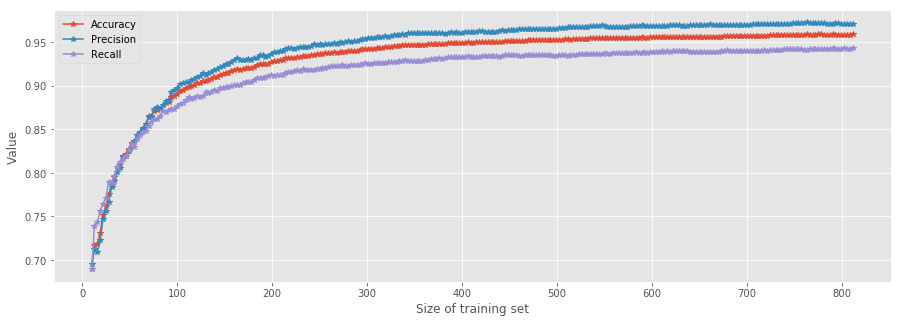
\includegraphics[scale = 0.28]{image/decisionLearning.png}
	\caption{Learning with Different size Data for Mushroom}
	\label{fig:treelearn}
\end{figure} 

\begin{figure}[h]
	\centering
	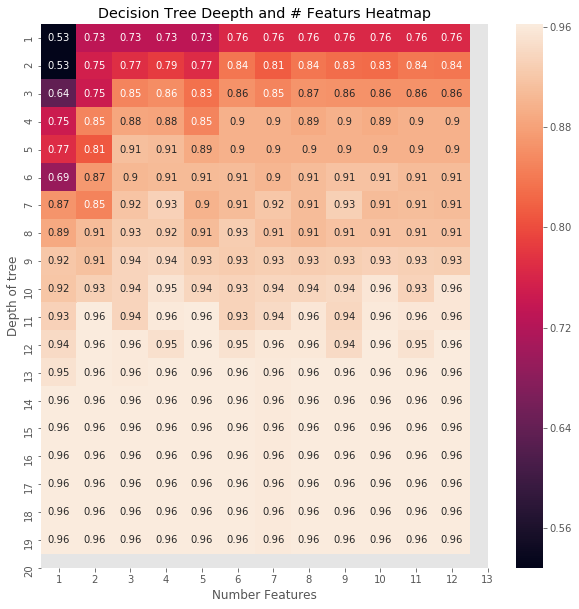
\includegraphics[scale = 0.28]{image/DTheatMap_mushroom.png}
	\caption{Model Accuracy Heatmap for Mushroom Data}
	\label{fig:mush_heat}
\end{figure}

\begin{figure}[h]
	\centering
	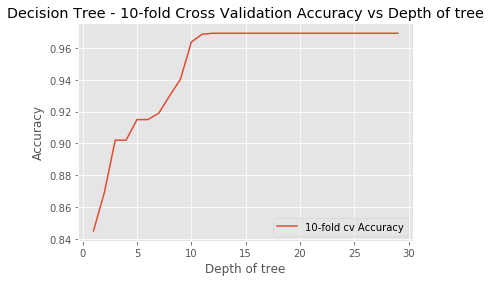
\includegraphics[scale = 0.5]{image/DT_MushRoom_crossValidation.png}
	\caption{Cross Validation Curve for Mushroom Dataset }
	\label{fig:mush_cv}
\end{figure}
Figure \ref{fig:mush_heat} is the accuracy heat map, the x axis is the number of features, and the y axis is the depth of the tree. According to this graph, the accuracy stop increase even after 13 lairs. However, the accuracy is not decreased also. Thant means the model is not overfitting even we push 20 lairs depth of tree node. This has been verified by cross-validation figure \ref{fig:mush_cv} also. the accuracy stop increase after around 13. After 13, the accuracy becomes a straight line.\\
\textit{\textbf{Analysis summary:}} Decision tree for this data set performance very good, the tree not overfitting by using too much data set, too deep, and too many features. This is because the feature to determine the 'class' is very obvious. In this case, too believe to the model is ok for predicting the class. 

\subsubsection{Decision Tree for Bank Dataset}
The bank behaves differently compared with the mushroom dataset. The best score I can get to predict the success by using the decision tree is 90.00\$ by using max deoth 7 and max features 11(best result come form the GridSearchCV method). However, 11.7\% of the bank data classified as 'yes', our decision tree method only better than just guessing 'No' a little bit. Still, the decision tree is better than random guessing 'Yes' and 'No'. Let discuss what performance graph is for this data set. \\
\begin{figure}[h]
	\centering
	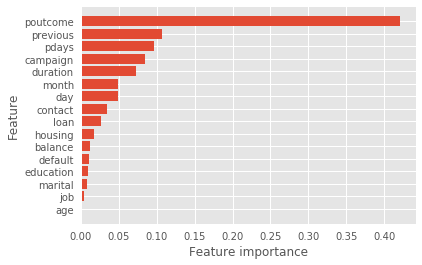
\includegraphics[scale = 0.5]{image/bank_important.png}
	\caption{Feature Importance for Bank Dataset }
	\label{fig:bank_dt_important}
\end{figure}
First, let us find out what feature is the most important for bank data. The feature 'poutcome' become the most important feature using in the classification, which has 'gini' index more than 0.43. Figure \ref{fig:bank_dt_tree} is a smaller version of the decision tree. We can check the top node is not the 'poutcome', this feature probability used in the down level. 
\begin{figure}[h]
	\centering
	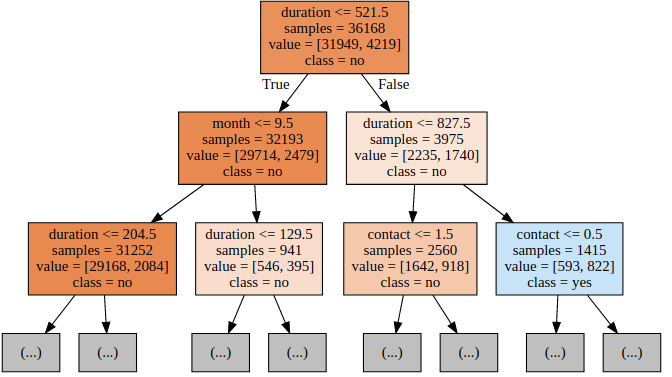
\includegraphics[scale = 0.3]{image/bank_dt_tree.png}
	\caption{Best Score Decision Tree for Bank Dataset }
	\label{fig:bank_dt_tree}
\end{figure}
Figure \ref{fig:bank_dt_learning} is the learning curve by using different data size. The accuracy increase dramatically in the beginning. One of the reason is the data set is not balanced. For example, just guess 'No' will also get a high accuracy. So the high learning rate is because the unbalanced data. \\
Other thing is the recall and precision curve is very low compare with the accuracy curve. This is also because the unbalanced data, which means the model did not predict the false positive very will. \\
\begin{figure}[h]
	\centering
	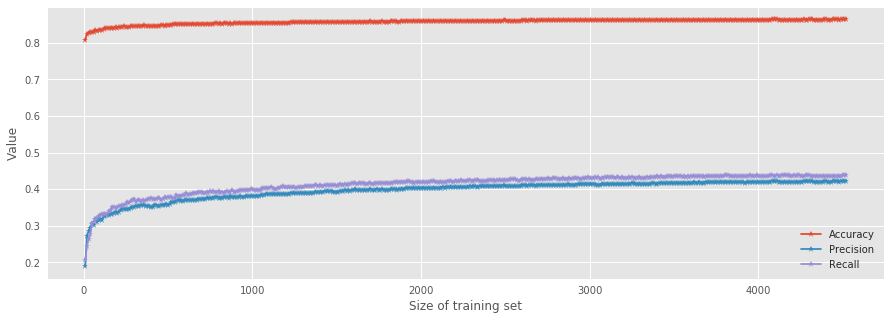
\includegraphics[scale = 0.2]{image/bank_dt_learning.png}
	\caption{Bank data learning curve }
	\label{fig:bank_dt_learning}
\end{figure}

\begin{figure}[h]
	\centering
	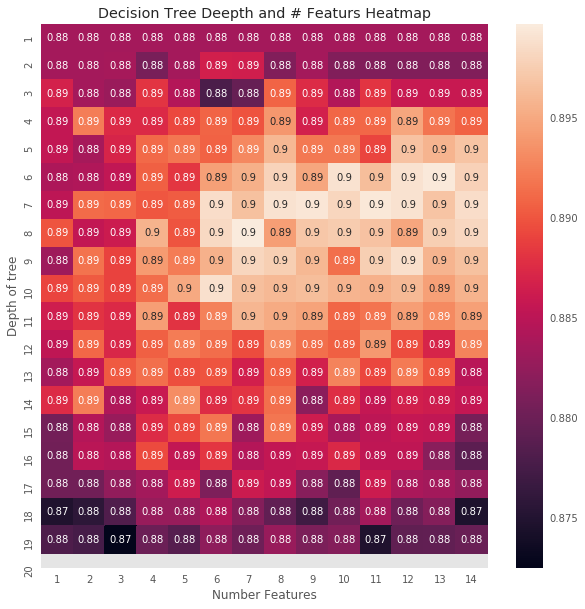
\includegraphics[scale = 0.4]{image/bank_dt_heat.png}
	\caption{DT Model Accuracy Heat Map for Bank Dataset  }
	\label{fig:bank_dt_heat}
\end{figure}
Figure \ref{fig:bank_dt_heat} gives us the accuracy heat map for a different number of features and depth of the tree. From this figure, we can find out the high accuracy is not at the bottom right as mushroom data. The high accuracy is in the middle of the graph. The reason is overfitting. By using too complicated data, the mode becomes too believe the training data set and become too complicated. 

\begin{figure}[h]
	\centering
	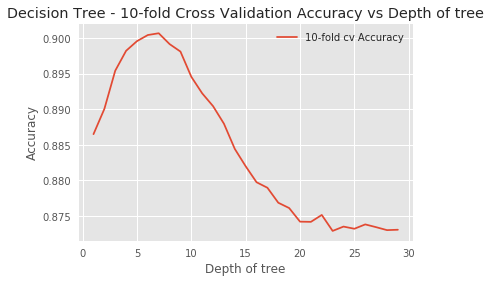
\includegraphics[scale = 0.5]{image/Bank_dt_cv.png}
	\caption{Cross Validation Curve for Bank Dataset  }
	\label{fig:bank_dt_cv}
\end{figure}
Figure \ref{fig:bank_dt_cv} shows the cross-validation curve for depth of the tree. From this curve, we can easily find out the tree overfitting the after the depth larger than 7. The accuracy decrease by using more complex model. We got the same result by using the heat map Figure \ref{fig:bank_dt_heat}. \\
\textit{\textbf{Analysis summary:}}Decision tree for this data set performance is not very good, however, the performance is much better than random guessing. The tree is nor overfitting with too much data set, however, the tree overfitted by using a large number of features and depth also. form this graph we can find out the power of cross-validation.

\subsection{Boosting}
The booing method will use AdaBoost method from Scikit learn library.An AdaBoost classifier is a meta-estimator that begins by fitting a classifier on the original dataset and then fits additional copies of the classifier on the same dataset but where the weights of incorrectly classified instances are adjusted such that subsequent classifiers focus more on difficult cases\cite{boost}.
\subsubsection{Boosing for Mushroom Dataset}
Using the Boosting method for the Mushroom data performs pretty good which give the same accuracy score compare with the decision tree method, the accuracy is 96.18\%. Boosting method is based on the decision tree method, in this implementation, I have set the limitation for the depth to 3 and max\_feature to 5.\\
Most of the performance is quite same with the decision tree. For example the important feature according to Figure \ref{fig:mush_abd_import}. For this data set, I did not find too much interesting performance compare boosting result with the decision tree method. However, the boosting take much longer to train and predict. 
\begin{figure}[h]
	\centering
	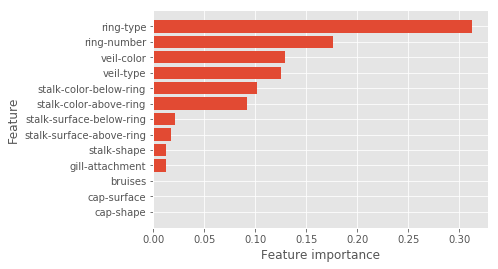
\includegraphics[scale = 0.5]{image/abd_feature_important.png}
	\caption{AdaBoost Feature Importance Graph for Mushroom}
	\label{fig:mush_abd_import}
\end{figure}
Figure \ref{fig:mush_abd_learing} is the testing accuracy compare with different training data size. Boosting method performance is similar with the decision tree. Figure \ref{fig:mush_heat} is the testing accuracy heat map, from this heat map, we can easily found out the model perform very well even we use small number of estimator and low learning rate. This means the AdaBoosting method perform very even without the cross validation. So for this question, no need to talk about the cross validation. 
\begin{figure}[h]
	\centering
	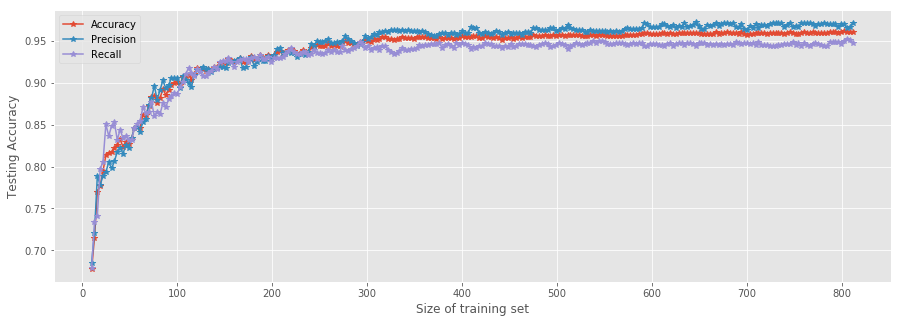
\includegraphics[scale = 0.3]{image/mush_abd_learning.png}
	\caption{AdaBoost Learning with different training data set for Mushroom}
	\label{fig:mush_abd_learing}
\end{figure}

\begin{figure}[h]
	\centering
	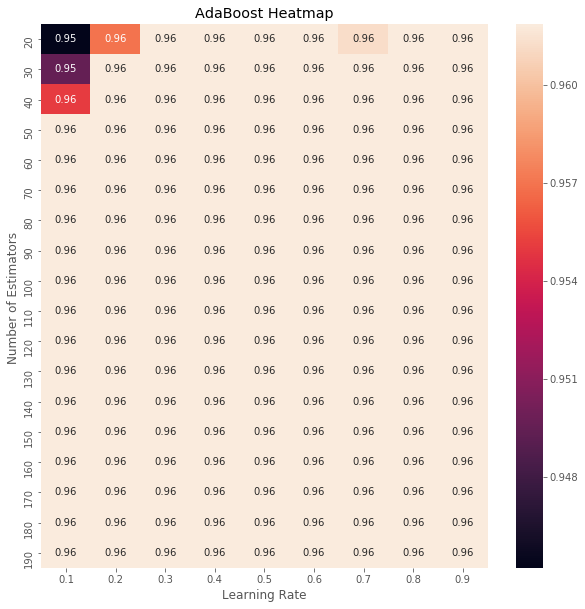
\includegraphics[scale = 0.3]{image/mush_abd_heat.png}
	\caption{AdaBoost Estimator and Learning rate Heat Map for Mushroom}
	\label{fig:mush_abd_heat}
\end{figure}

\textit{\textbf{Analysis summary:}} The AdaBoost method preform very well, even without too much parameter tunning. This is also one of the advantage of Boosting method. Is this true for every data set or only for this particular dataset. Let us find out in the bank data set in next section.

\subsubsection{Boosing for Bank Dataset}
The boosting method for bank dataset perform better than the decision tree method, The best accuracy score I can get for this dataset is 90.48\%, but the training and testing time longer than the decision tree method. From figure \ref{fig:bank_abd_important} importance feature map, is a little bit different than the Figure \ref{fig:bank_dt_important}. For the decision tree, the 'poutcome' feature dominate the classification, however, for the boosting method, almost all the feature contribute to the classification. 
\begin{figure}[h]
	\centering
	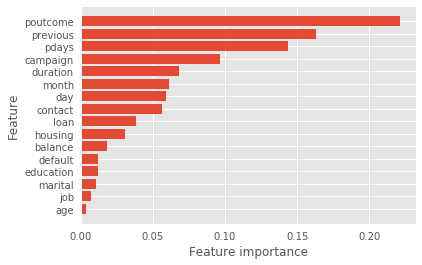
\includegraphics[scale = 0.5]{image/bank_abd_important.png}
	\caption{AdaBoost Estimator and Learning rate Heat Map for Bank}
	\label{fig:bank_abd_important}
\end{figure}

The learning curve performs a little bit different compared with the decision tree which is Figure \ref{fig:bank_dt_learning}. Especially for the precision curve, it keep increase pass 0.52

\begin{figure}[h]
	\centering
	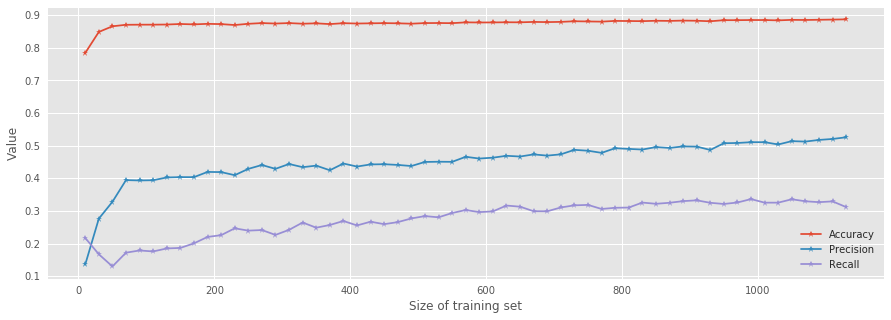
\includegraphics[scale = 0.25]{image/bank_abd_learning.png}
	\caption{AdaBoost Learning with different training data set for Bank}
	\label{fig:bank_abd_learing}
\end{figure}

Also the heat map figure \ref{fig:bank_abd_heat}, also indicate the mode is not easy to overfitting. with number increased, the testing data did not drop. Compare with the decision tree method, which easily gets over fitted by using the deeper decision tree. The  best value get from GridSearchCV() is with 80 estimators, and learning rate is 0.3. 

\begin{figure}[h]
	\centering
	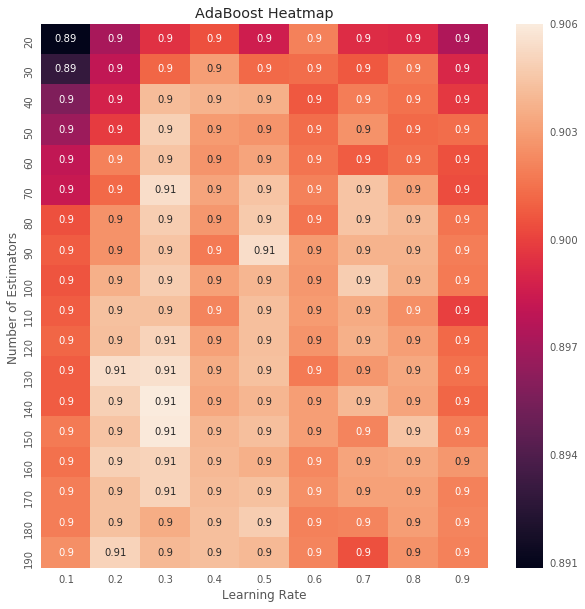
\includegraphics[scale = 0.3]{image/bank_abd_heat.png}
	\caption{Estimator and Learning rate Heat Map for Bank }
	\label{fig:bank_abd_heat}
\end{figure}

For the cross-validation test, I have designed two cases. One is keep the learning rate the same and get 10 folder validation accuracy for estimator [2,100], which is the figure \ref{fig:bank_abd_cros_est}. For this figure, we can understand the number of the estimator did not overfit the model. With the number of estimator increase, the accuracy increase. However, the accuracy increasing rate become much slower at 80. 

\begin{figure}[h]
	\centering
	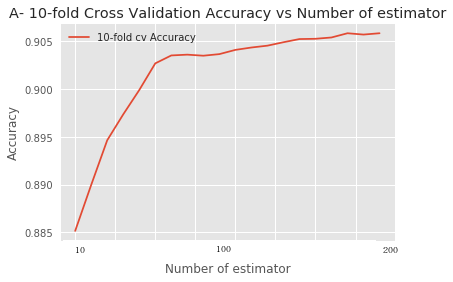
\includegraphics[scale = 0.5]{image/bank_abd_cross_est.png}
	\caption{Cross Validation Score for Number of Estimator for Bank}
	\label{fig:bank_abd_cros_est}
\end{figure}

Figure \ref{fig:bank_abd_cros_rate} is the boosting learning rate from [0.1 to 1.0]. However, from this figure, we can easily find out the model do over with learning rate larger than 0.3. This is a very interesting graph to show that, fine tune the learning rate is very important for some of the machine learning algorithms. 

\begin{figure}[h]
	\centering
	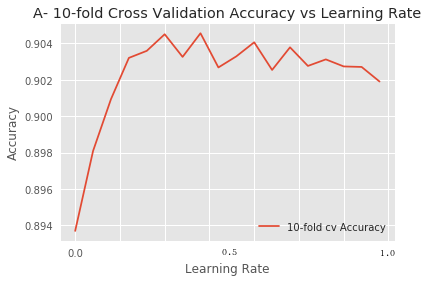
\includegraphics[scale = 0.5]{image/bank_abd_cross_rate.png}
	\caption{Cross Validation Score for Learning Rate for Bank}
	\label{fig:bank_abd_cros_rate}
\end{figure}

\textit{\textbf{Analysis summary:}} The AdaBoost method performs much better than the pure decision tree method. Using the same training and testing set, the accuracy increased almost 1.5\% which is pretty good for large problems. And the overfitting problem is very well handled by using this method. We only need to set a good learning rate. However, this method is very slow, for detailed comparison, please check the last part of this report. As a method based on the decision tree, boosting method out preform decision tree in terms of the testing accuracy. 

\subsection{Neural Network}
Advantages of neural networks include their high tolerance to noisy data, as well as their ability to classify patterns on which they have not been trained. The most popular neural network algorithm is the back-propagation algorithm\cite{neural}.
Neural Network is quite popular in recent years, due to the deep neural network structure improved the machine problem a lot, especial for the large unstructured dataset. For this algorithm, there are quite a lot parameters can be tuned. For example, number of hidden layers, number of the neuron for each hidden layer, different activation function, different solver functions, and different learning rate. For this section of this report, I will keep some of the parameters the same, 2 hidden layers and each of the layer will using the same number of nodes. 
\subsubsection{Neural Network for Mushroom Dataset}
The performance of the Neural Network for the mushroom dataset is not that great compared with the previous two methods. The best testing score I can get is 94.89\%. I think one of the reason is the neural network is very good for unstructured data for example voice, image. For this simple classification problem, it does not a suitable model. \\
The analysis is from the previous section. The first graph will be the number of samples used and testing accuracy. Figure \ref{fig:mush_nn_learing} is the figure for different size of training set. The data is based on two 30 nodes hidden layer and use 'real'. The accuracy both of training and testing become periodic. Every 200 samples, the accuracy decreased a lot. This probability according to the max interaction settled to 200. From this picture, we find out the neural network model is sensitive to the parameter. After the neural network has been build, during the training the structure can not change any more.  
 
\begin{figure}[h]
	\centering
	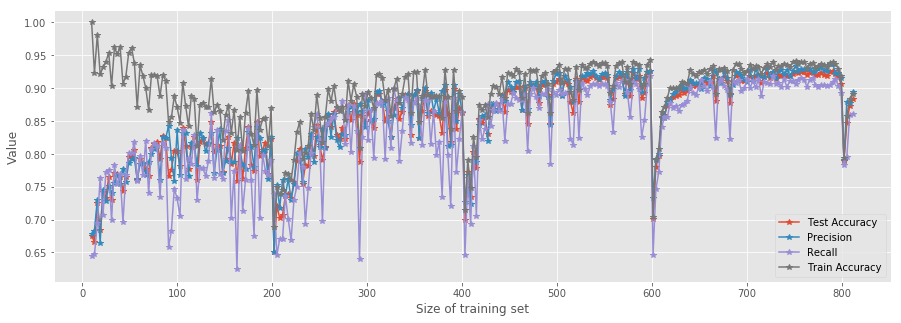
\includegraphics[scale = 0.25]{image/mush_nn_learning.png}
	\caption{Neural Network with Different Size Training Set for Mushroom}
	\label{fig:mush_nn_learing}
\end{figure}

Figure \ref{fig:mush_nn_learing_rate} is the 10 folder cross validation testing for learning rate. The learning rate is from 0.001 to 0,05. From this graph, we can easily discover the large number of learning rate decrease the testing accuracy. The solver in this case is 'adam'. 

\begin{figure}[h]
	\centering
	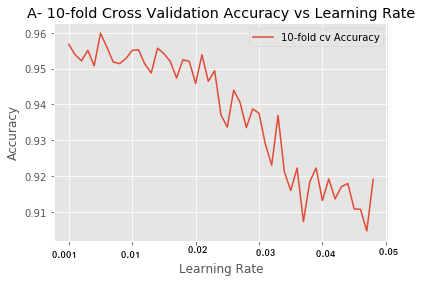
\includegraphics[scale = 0.5]{image/mush_nn_learning_rate.png}
	\caption{Cross Validation for Different Learning Rate for Mushroom}
	\label{fig:mush_nn_learing_rate}
\end{figure}

For the model complexity analysis, I have select tow parameter for cross-validation analysis. On is the max iteration and an other is the size of two hidden layer. Figure \ref{fig:mush_nn_learing_maxIter} is the max iteration curve. The range of the iteration is from 20 to 300. From this curve, the accuracy after 120 stop changing. I think the reason is because the model converge after 120. Even tough, the max iteration has been set to large number, the accuracy won't change. 
\begin{figure}[h]
	\centering
	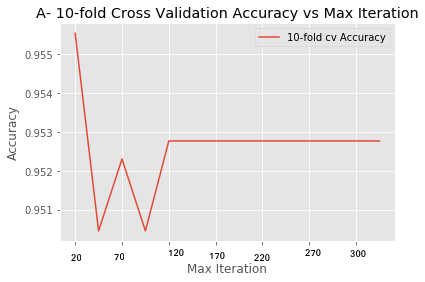
\includegraphics[scale = 0.5]{image/mush_nn_maxiteration.png}
	\caption{Cross Validation for Different Learning Rate for Mushroom}
	\label{fig:mush_nn_learing_maxIter}
\end{figure}

Figure \ref{fig:mush_nn_learing_layer} is the size of each hidden layer and cross-validation accuracy. From this curve, the accuracy increase in the begin, which means 2*2 is not complex enough to handle this problem. After 10 by 10, the model is good enough for this classification problem because the accuracy stop increase after size of 10. 

\begin{figure}[h]
	\centering
	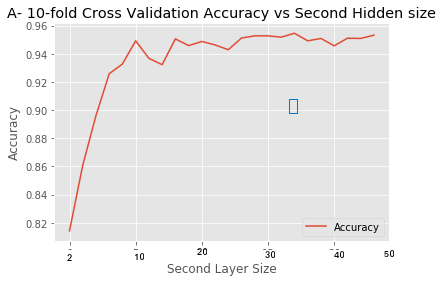
\includegraphics[scale = 0.5]{image/mush_nn_layerSize.png}
	\caption{Cross Validation for Different Learning Rate for Mushroom}
	\label{fig:mush_nn_learing_layer}
\end{figure}
\subsubsection{Neural Network for Bank Dataset}
For the bank data set, the neural network did not preform very well as the previous problem. The best training score I got for this problem is 89.10\%. Let discover some of the performance of this model. Figure \ref{fig:bank_nn_learing} is compare with different training size and testing/ training accuracy. This is quite different from the previous result. The recall accuracy drop to 0, this means the algorithm just predict 'No' all the time. 

\begin{figure}[h]
	\centering
	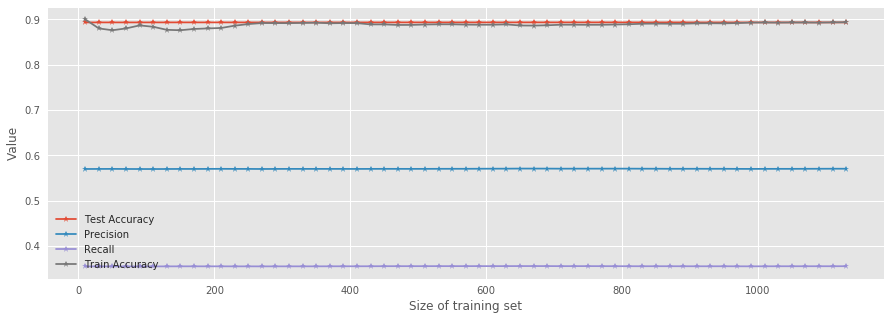
\includegraphics[scale = 0.25]{image/bank_nn_learning.png}
	\caption{Neural Network with Different Size Training Set for Bank Data}
	\label{fig:bank_nn_learing}
\end{figure}

Figure \ref{fig:bank_nn_learing_rate} is the relation between the learning rate and the cross-validation accuracy. From this curve, the model accuracy stop around 88.80\%. This is the same accuracy you can get by only predict 'No'. In this case, the Neural Network in this particular problem is same will just saying 'No' to every one. This probability because, the neural network is not good to handle the unbalanced datasets. 
 
\begin{figure}[h]
	\centering
	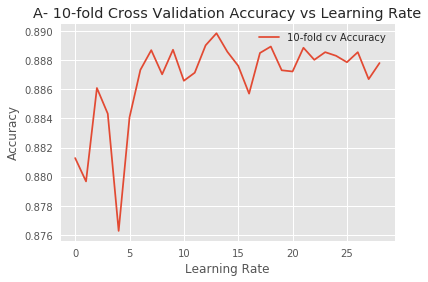
\includegraphics[scale = 0.5]{image/bank_nn_learning_rate.png}
	\caption{Cross Validation for Different Learning Rate for Bank Data}
	\label{fig:bank_nn_learing_rate}
\end{figure}

Figure \ref{fig:bank_nn_layer} is the hidden layer size and accuracy, from this curve, we got a similar result with other assumption. The size of hidden is not affecting the accuracy too much, and the model still not working very well. 

\begin{figure}[h]
	\centering
	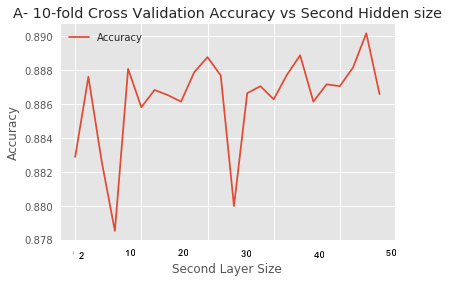
\includegraphics[scale = 0.5]{image/bank_nn_layersize.png}
	\caption{Cross Validation for Different Learning Rate for Bank Data}
	\label{fig:bank_nn_layer}
\end{figure}
\textit{\textbf{Analysis summary:}} In this section, neural network method has been used for this two classification problem. However, no matter what parameter I have change neural network refuse to perform well. In conclusion, neural network probability is not good for this kind of classification problem. 

\subsection{Support Vector Machine(SVM)}
Support vector machines (SVMs) are a set of supervised learning methods used for classification, regression and outliers detection. The advantages of support vector machines are Effective in high dimensional spaces, versatile: different Kernel functions. \\
The SVM is also a very complex machine learning model. However, compare with the deep neural network, still, have much less learning parameter. For example, different kernel, degree, max\_iter. In this assignment, I will use the mushroom and bank data to test the performance some of these tuning parameters. Let us start with the mushroom first.

\subsubsection{SVM for Mushroom Dataset}
One of the things I need to mention when I use the SVM is slow. The algorithm performs very slow. Both training and testing. The best testing accuracy I can get from this machine learning method is 96.18\%. Two kernel functions have been used for testing the learning curve, which 'rbf' and 'ploy' with degree 3.\\
Figure \ref{fig:mushroom_svm_learning_rbf} is the learning curve with different input size data for 'rbf' kernel. Figure \ref{fig:mushroom_svm_learning_pol} is the learning curve for polynomial kernel with degree 3. From this two graph, we can get some knowledge about these two kernels. The polynomial function with degree 3 is much simpler than rbf kernel. that is probably better for low dimension problem. 

\begin{figure}[h]
	\centering
	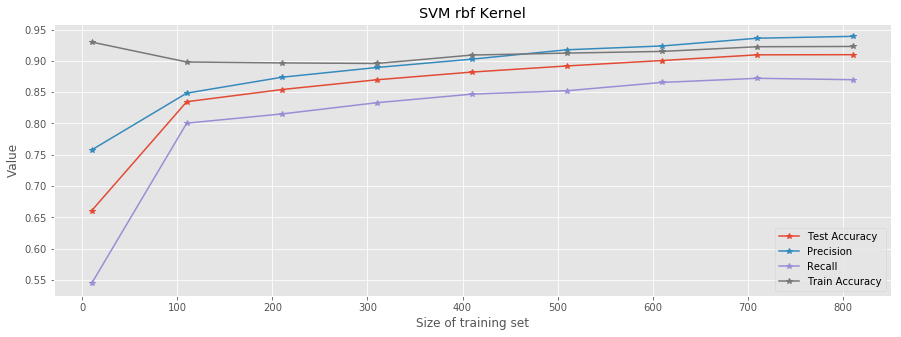
\includegraphics[scale = 0.25]{image/mush_svm_learning_rbf.png}
	\caption{SVM rbf Kernel Learning Curve vs Number of Samples for Mushroom}
	\label{fig:mushroom_svm_learning_rbf}
\end{figure}  

\begin{figure}[h]
	\centering
	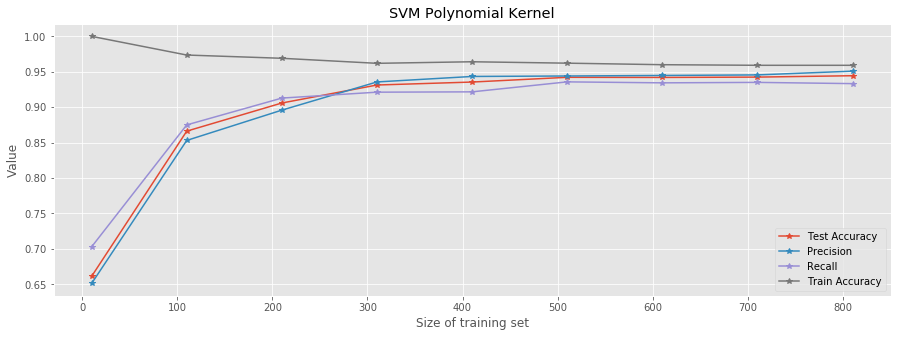
\includegraphics[scale = 0.25]{image/mush_svm_learning_pol.png}
	\caption{SVM Polynomial Kernel Learning Curve vs Number of Samples for Mushroom}
	\label{fig:mushroom_svm_learning_pol}
\end{figure}  

For the model complexity problem, the experiment I have designed is the order or polynomial order. Figure \ref{fig:mushroom_svm_pol} is the different polynomial order and accuracy comparison. For this curve, the testing and training accuracy stop increasing after 3 order, which means the oder 3 is good enough for handle this problem. 

\begin{figure}[h]
	\centering
	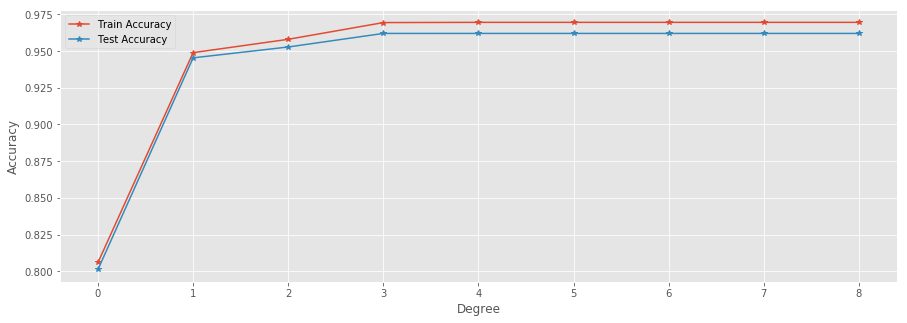
\includegraphics[scale = 0.25]{image/mush_svm_polynomial.png}
	\caption{SVM Polynomial Order and Accuracy for Mushroom}
	\label{fig:mushroom_svm_pol}
\end{figure} 


\subsubsection{SVM for Bank Dataset}
The SVM algorithm for this problem is very slow. I have to reduce the training data set in order to plot some of the graph. The best testing score I can get from SVM is 88.4. The algorithm is quite slow especially for this large dataset. I can not massively run the model to generate such a learning graph using this Banks data. For analysis, I believe the performance of this model is the same with the mushroom dataset. 

\textit{\textbf{Analysis summary:}} the SVM is a very computational expensive algorithm. In order to plot some of the graph, I have to reduce the training data size. 

\subsection{ K Nearest Neighbors(KNN)}
 Nearest neighbors provide functionality for unsupervised and supervised neighbors-based learning methods. The principle behind nearest neighbor methods is to find a predefined number of training samples closest in distance to the new point, and predict the label from this \cite{nn}.\\ 
The KNN classification is a type of instance-based learning: it does not attempt to construct a general internal model, but simply stores instances of the training data. Classification is computed from a simple majority vote from K nearest neighbors. The algorithm run very fast, as fast as decision tree method. One interesting thing about this method is the running time between the training and predicting. Because this is a slow learner, the predicting take some additional work.\\
Compare with other machine learning method, KNN is quite simple. It has only a few parameters, for example, number of neighbors, the weight of each sample. The KNN algorithm has been applied to the two datasets. Let us start with the mushroom data.

\subsubsection{KNN for Mushroom Dataset}
The result of the KNN algorithm for this data set is very good, the best score I can get is 96.06\% for the testing dataset. Let us check out the relation between training sample size and training/testing data.\\
Figure \ref{fig:mushroom_knn_learning} is the learning curve. From this curves, it is easy to find out, the training curve is very high and the testing is very low at first.This is normal for most of the machine learning algorithm. However, for KNN the reason is little bit difference Because, for the small number of sample points, the algorithm to believe the data, and there are only a few of them. So at the beginning, the training accuracy decrease, and testing accuracy increase dramatically. After 500 sample point, the accuracy increase becomes very slow means, this model becomes mature.  More samples will not contribute to the model too much. 

\begin{figure}[h]
	\centering
	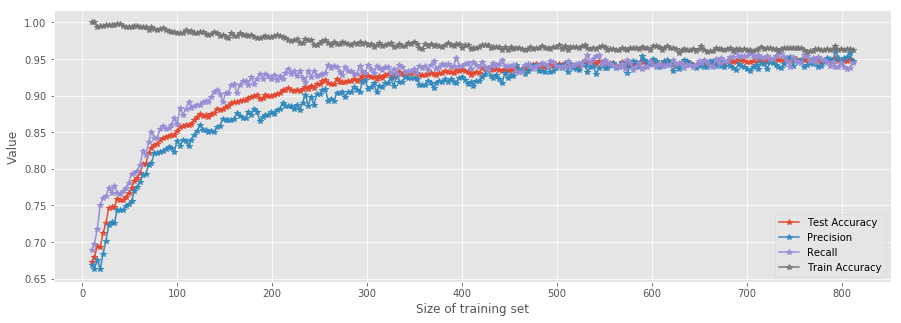
\includegraphics[scale = 0.25]{image/mushroom_knn_learning.png}
	\caption{KNN Learning Curve vs Number of Samples for Mushroom}
	\label{fig:mushroom_knn_learning}
\end{figure}

For the KNN mode, I have only designed one test case to analyze the model complexity. In terms of the model complexity for KNN is the number of neighbors. So in this part, the cross-validation score for different K score shown in figure \ref{fig:mushroom_knn_K}. In this figure, there are two curves, one for uniform sample weight, another weight is based on the distance. From these tow performance curves, we can assume the uniform weight over-fit when K increase over 10 neighbors. When three are lots of neighbors, even some of the neighbors from long distance, we can assume the irrelevance sample point involved for the final result .if every one contributes the same weight the model easy to over-fit. However, for the weight based on the distance, it makes sense when the point for away involved in the final result. 

\begin{figure}[h]
	\centering
	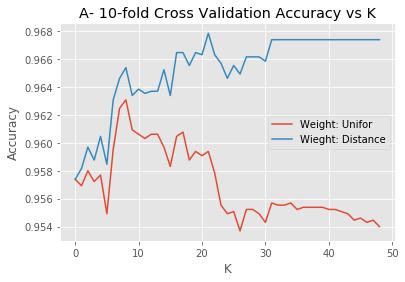
\includegraphics[scale = 0.5]{image/mushroom_knn_K.png}
	\caption{Cross Validation for Different K for Mushroom}
	\label{fig:mushroom_knn_K}
\end{figure}

\subsubsection{KNN for Bank Dataset}

This section will discuss the KNN for Bank Dataset. The kNN give us an ok result, the testing accuracy I got is 88.18\%. It is common for most of the algorithm. The learning curve is in figure \ref{fig:bank_knn_learning}, the training curve is always higher than the testing accuracy. The recall accuracy keeps running low, which means the prediction was not great on the "Yes" class. We got a similar result compared with a neural network. However, for the neural network, the training and testing accuracy stays the same.

\begin{figure}[h]
	\centering
	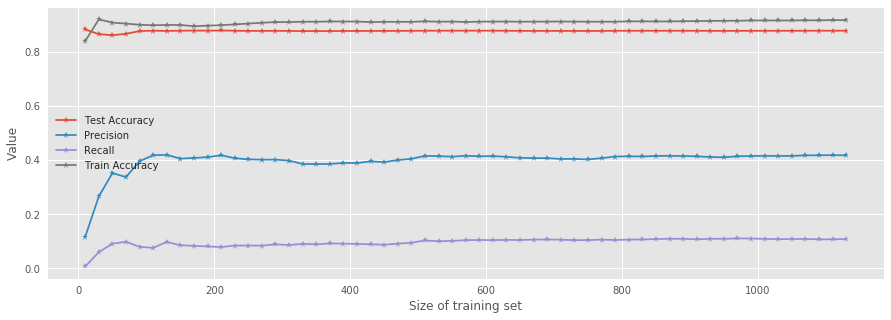
\includegraphics[scale = 0.25]{image/bank_knn_learning.png}
	\caption{KNN Learning Curve vs Number of Samples for Bank}
	\label{fig:bank_knn_learning}
\end{figure}

Figure \ref{fig:bank_knn_K} is the cross-validation accuracy and K. Compare with the mushroom data, the model accuracy did not decrease. One of the reason is that this is an unbalanced dataset. If we increase the K to the number of training samples, the accuracy would become the majority class all the time. Because the majority of the sample is one class. This probability happed to this dataset. The accuracy stay the portion of "No" class for the training sets.

\begin{figure}[h]
	\centering
	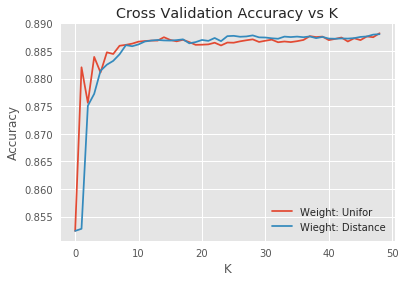
\includegraphics[scale = 0.5]{image/bank_knn_learning_k.png}
	\caption{Cross Validation for Different K for Bank}
	\label{fig:bank_knn_K}
\end{figure}

\textit{\textbf{Analysis summary:}} the algorithm run very quick, and the result pretty good also. For kNN, the model is not complex, and there are no optimization method involved during the training and testing. Some advanced data structures have been involved, for example KD tree to reduce the complexity. 
\section{Result Analysis and Comparison}
In this section, I will compare with different machine learning algorithm. There are two comparison, one is testing accuracy, another is the training time. The testing and training data set is the same for comparison. 80\% for training and 20\% for testing. 

\subsubsection{Testing Dataset Accuracy}
Table \ref{tab:accuracy} is the accuracy comparison for these five different algorithm. For some computational expensive method I did not use the GridSearchCV method to find the best parameter. There are some difference between different algorithm. For mushroom data set, three algorithms give the same answer. For the bank dataset, the boosting method got the best testing accuracy.\\
Boosting is an improved version of decision tree. So the result better than decision tree is quire normal. However, the computation is mush expensive than decision tree, which talk in detail in next section. 

\begin{table}[h]
	\centering
	\caption{Testing Dataset Accuracy}
	\label{tab:accuracy}
	\begin{tabular}{|l|c|c|c|c|c|}
		\hline
		Data Set & DT      & Boost   & Neural Net & SVM     & KNN     \\ \hline
		Mushroom & 96.18\% & 96.18\% & 94.40\%    & 96.18\% & 96.06\% \\ \hline
		Bank     & 90.00\% & 90.47\% & 88.85\%    & 88.45\% & 88.76\% \\ \hline
	\end{tabular}
\end{table}

\subsubsection{Training and Testing Time}
In this section, I will talk about the training and testing time for those five different algorithms. Table \ref{tab:time} is the training and testing time for five different machine learning algorithm.\\
In terms of training time, a decision tree is the best, and SVM is the worst algorithm. Decision tree and KNN did not involve complex optimization algorithm, so that is one of the reasons it performs very well. \\
In terms of the testing time. the decision tree also the best algorithm, KNN become the worst one. I just mentioned in the KNN section. KNN is a slow learner, which means the KNN put the computing during the predicting period. KNN is also the only algorithm which the testing time is more than the training time. 
 \begin{table}[h]
 	\centering
 	\caption{Mushroom Data Testing and Training Time (second)}
 	\label{tab:time}
 	\begin{tabular}{|l|c|c|c|c|c|}
 		\hline
 		Mushroom & DT     & Boost  & Neural Net & SVM    & KNN    \\ \hline
 		Training & 0.0052 & 0.5027 & 3.0978     & 7.3608 & 0.0115 \\ \hline
 		Testing  & 0.0008 & 0.0275 & 0.0017     & 0.0681 & 0.1192 \\ \hline
 	\end{tabular}
 \end{table}

\section{Conclusion}
In this report, I have discussed five supervised learning method and results from two datasets in detail. Some of the algorithms are very simple, for example, decision tree and kNN, some of the algorithms involved lots of optimization and calculation, for example, neural network. They all have their characteristic also. Without knowing the fundamental knowledge, you can not understand the result of a particular algorithm, or how to improve it. \\

This is the end of this report, I would like to thank for this open end assignment. Typically you can spend the infinite time to work on this. For the time constraint, this would be all I have. I am glad I did this. 



% trigger a \newpage just before the given reference
% number - used to balance the columns on the last page
% adjust value as needed - may need to be readjusted if
% the document is modified later
%\IEEEtriggeratref{8}
% The "triggered" command can be changed if desired:
%\IEEEtriggercmd{\enlargethispage{-5in}}

% references section

% can use a bibliography generated by BibTeX as a .bbl file
% BibTeX documentation can be easily obtained at:
% http://www.ctan.org/tex-archive/biblio/bibtex/contrib/doc/
% The IEEEtran BibTeX style support page is at:
% http://www.michaelshell.org/tex/ieeetran/bibtex/
%\bibliographystyle{IEEEtran}
% argument is your BibTeX string definitions and bibliography database(s)
%\bibliography{IEEEabrv,../bib/paper}
%
% <OR> manually copy in the resultant .bbl file
% set second argument of \begin to the number of references
% (used to reserve space for the reference number labels box)
{\footnotesize \bibliographystyle{IEEEtran}
\bibliography{references}}

%\begin{thebibliography}{1}
%
%\bibitem{IEEEhowto:kopka}
%H.~Kopka and P.~W. Daly, \emph{A Guide to \LaTeX}, 3rd~ed.\hskip 1em plus
%  0.5em minus 0.4em\relax Harlow, England: Addison-Wesley, 1999.
%
%\end{thebibliography}




% that's all folks
\end{document}


